\documentclass{article}

\usepackage{fullpage}
\usepackage{color}
\usepackage{amsmath}
\usepackage{url}
\usepackage{verbatim}
\usepackage{graphicx}
\usepackage{parskip}
\usepackage{amssymb}
\usepackage{nicefrac}
\usepackage{listings} % For displaying code
\usepackage{algorithm2e} % pseudo-code

% Answers
\def\ans#1{\par\gre{Answer: #1}}
%\def\ans#1{} % Comment this line to produce document with answers

% Colors
\definecolor{blu}{rgb}{0,0,1}
\def\blu#1{{\color{blu}#1}}
\definecolor{gre}{rgb}{0,.5,0}
\def\gre#1{{\color{gre}#1}}
\definecolor{red}{rgb}{1,0,0}
\def\red#1{{\color{red}#1}}
\def\norm#1{\|#1\|}

% Math
\def\R{\mathbb{R}}
\def\argmax{\mathop{\rm arg\,max}}
\def\argmin{\mathop{\rm arg\,min}}
\newcommand{\mat}[1]{\begin{bmatrix}#1\end{bmatrix}}
\newcommand{\alignStar}[1]{\begin{align*}#1\end{align*}}

% LaTeX
\newcommand{\fig}[2]{\includegraphics[width=#1\textwidth]{a1f/#2}}
\newcommand{\centerfig}[2]{\begin{center}\includegraphics[width=#1\textwidth]{a1f/#2}\end{center}}
\def\items#1{\begin{itemize}#1\end{itemize}}
\def\enum#1{\begin{enumerate}#1\end{enumerate}}
\newcommand{\matCode}[1]{\lstinputlisting[language=Matlab]{a1f/#1.m}}


\begin{document}

\title{CPSC 340 Assignment 1 (due Friday September 29 ATE)}
\author{}
\date{}
\maketitle
\vspace{-4em}

The assignment instructions are the same as Assignment 0, except you have the option to work in a group of 2. If you work in a group, please only hand in \emph{one} assignment. It is recommended that you work in groups as the assignment is quite long, but please only submit one assignment for the group and make sure that everyone's name/ID is on the front page.


\section{Summary Statistics and Data Visualization}

Download and expand the file \emph{a1.zip}, which contains estimates of the influenza-like illness percentage over 52 weeks on 2005-06 by Google Flu Trends in a comma-separated values (CSV) file. You can open this with Excel or other spreadsheet programs; the first row gives the abbreviation of the region names for each column, and each row gives the estimate for a week.
After you change to the a0 directory, you can load this data in Julia using:
\begin{verbatim}
dataTable = readcsv("fluTrends.csv")
\end{verbatim}
This creates an two-dimensional array of type ``Any''  populated with all the information in the CSV file.

\subsection{Summary Statistics}

\blu{Report the following statistics}: the minimum, maximum, mean, median, and mode of all values across the dataset. In light of thea above, \blu{is the mode a reliable estimate of the most ``common" value? Describe another way we could give a meaningful ``mode" measurement for this (continuous) data.}

Hint: Since the first row of the CSV file is just the names of the columns, we can create a matrix $X$ containing the data stored as real numbers using:
\begin{verbatim}
X = real(dataTable[2:end,:])
\end{verbatim}
Also, Julia has no mode command so I've included a mode function in `misc.jl'.


\subsection{Data Visualization}

Consider the figure on the next page.
The figure contains the following plots, in a shuffled order:
\enum{
\item A histogram showing the distribution of each the values in the matrix $X$.
\item A boxplot grouping data by weeks, showing the distribution across regions for each week.
\item A scatterplot between the two regions with highest correlation.
\item A single histogram showing the distribution of \emph{each} column in $X$.
\item A scatterplot between the two regions with lowest correlation.
\item A plot containing the weeks on the $x$-axis and the percentages for each region on the $y$-axis.
}
\blu{Match the plots (labeled A-F) with the descriptions above (labeled 1-6), with an extremely brief (a few words is fine) explanation for each decision.}

Hint: you can generate similar plots by adding the PyPlot package. To add this package use:
\begin{verbatim}
Pkg.add("PyPlot") # Do this once per computer
using PyPlot # Do this once per session
plot(1:52,X[:,1]) # Plot the first row
\end{verbatim}
To generate similar-looking plots you can use the functions `plot', `boxplot', `plt[:hist]', and `scatter'.


\subsection{Decision Surfaces}

Consider the figure below, which plots a set of two-dimensional training examples and the decision surface produced by a ``neural network'' classifier (a model we'll see later in the course).
\blu{How many training examples has the neural network mis-classified?} (This figure is best viewed in colour.)

\section{Decision Trees}

\subsection{Equality vs. Inequality Splitting Rules}

It might make more sense when working with features with few, discrete values that are not related. For example, with 'colour' as a feature converted to numbers, inequalities wouldn't make a lot of sense as the numbers representing the colours are not related in quantity.

\subsection{Decision Stump Implementation}

Training Error of \texttt{decisionStump}: 0.25

\subsection{Constructing Decision Trees}
\begin{verbatim}
if latitude > 37.669007
    if longitude > -96.090109
        return 1
    else
        return 2
else
    if longitude > -155.577574
        return 2
    else
        return 1
\end{verbatim}



\subsection{Cost of Fitting Decision Trees}

The first (top-level) decision stump takes $O(nd\log{n})$ time, and as we split, the second-level decision stumps each takes $O(nd\log{\frac{n}{a}})$ and $O(nd\log{\frac{n}{b}})$ time, where $\frac{n}{a} + \frac{n}{b} = n$. So the second layer takes $O(nd\log{n})$ time still. We apply the same reasoning to each layer, and we have a total of $m$ layers, so the total cost is $O(mnd\log{n})$ time.

\section{Training and Testing}

\subsection{Training Error}

Initially, the training error of \texttt{decisionStump} decreases as the depth increases, but it stops decreasing after depth 4. On the other hand, the training error of infogain decreases with increasing depth all the way to zero.

The error stops decreasing after a certain depth for the decision tree model likely because the splitting isn't even and sometimes the NO case has no more objects even when there are still objects of different labels in the same YES case. When this happens, we have reached the base split case and our implementation of \texttt{decisionTree} will split no further, meaning that some of the objects that end up in the same YES-leaf have different labels, which means some of them will be assigned labels different from the actual labels they have, which increases the training error regardless of what value is assigned to them.

\subsection{Training and Testing Error Curves}

\textit{
Legend:
\begin{itemize}
	\item blue crosses are training errors
	\item red dots are test errors
	\item x-axis represents the depth
	\item y-axis represents the error
\end{itemize}}

\begin{figure}[h!]
  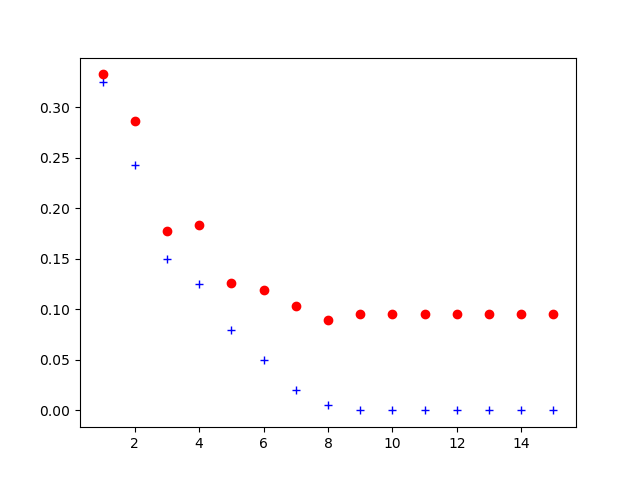
\includegraphics[height=7.5cm]{Etrain_Etest_vs_depth.png}
  \caption{Training Error and Test Error vs. Depth}
  \label{fig: error vs depth}
\end{figure}



\subsection{Validation Set}

If we split the dataset in half and use the first half for training and second half for validation, the minimum validation set error we were able to obtain was 0.165 at depth 4 with a 0.110 train error, but after depth 4 the validation set error stays the same. If we switch the data sets and use the second half for training and first half for validation, the minimum validation error becomes 0.155 at depth 4 with a 0.105 training error. To use more of our data to estimate depth, we could use cross validation so every object is used for validation once.

\section{Naive Bayes}

In this section we'll implement naive Bayes, a very fast classification method that is often surprisingly accurate for text data with simple representations like bag of words.



\subsection{Naive Bayes by Hand}

Consider the dataset below, which has $10$ training examples and $2$ features:
\[
X = \begin{bmatrix}0 & 1\\1 & 1\\ 0 & 0\\ 1 & 1\\ 1 & 1\\ 0 & 0\\  1 & 0\\  1 & 0\\  1 & 1\\  1 &0\end{bmatrix}, \quad y = \begin{bmatrix}1\\1\\1\\1\\1\\1\\0\\0\\0\\0\end{bmatrix}.
\]
Suppose you believe that a naive Bayes model would be appropriate for this dataset, and you want to classify the following test example:
\[
\hat{x} = \begin{bmatrix}1 & 0\end{bmatrix}.
\]

\blu{(a) Compute the estimates of the class prior probabilities} (you don't need to show any work):
\items{
\item$ p(y = 1)$.
\item $p(y = 0)$.
}

\blu{(b) Compute the estimates of the 4 conditional probabilities required by naive Bayes for this example}  (you don't need to show any work):
\items{
\item $p(x_1 = 1 | y = 1)$.
\item $p(x_2 = 0 | y = 1)$.
\item $p(x_1 = 1 | y = 0)$.
\item $p(x_2 = 0 | y = 0)$.
}

\blu{(c) Under the naive Bayes model and your estimates of the above probabilities, what is the most likely label for the test example? (Show your work.)}

\subsection{Bag of Words}

If you run the script \emph{example\_bagOfWods.jl}, it will load the following dataset:
\enum{
\item $X$: A sparse binary matrix. Each row corresponds to a newsgroup post, and each column corresponds to whether a particular word was used in the post. A value of $1$ means that the word occured in the post.
\item $wordlist$: The set of words that correspond to each column.
\item $y$: A vector with values $1$ through $4$, with the value corresponding to the newsgroup that the post came from.
\item $groupnames$: The names of the four newsgroups.
\item $Xvalidate$ and $yvalidate$: the word lists and newsgroup labels for additional newsgroup posts.
}
\blu{Answer the following}:
\enum{
\item Which word is present in the newsgroup post if there is a $1$ in column 50 of X?
\item Which words are present in training example 500?
\item Which newsgroup name does training example 500 come from?
}

\subsection{Naive Bayes Implementation}

If you run the function \emph{example\_decisionTree\_newsgroups.jl} it will load the newsgroups dataset and report the test error for decision trees of different sizes (it may take a while for the deeper trees, as this is a sub-optimal implementation). On other other hand, if you run the function \emph{example\_naiveBayes.jl} it will fit the basic naive Bayes model and report the test error.

While the \emph{predict} function of the naive Bayes classifier is already implemented, the calculation of the variable $p\_xy$ is incorrect (right now, it just sets all values to $1/2$). \blu{Modify this function so that \emph{p\_xy} correctly computes the conditional probabilities of these values based on the frequencies in the data set. Hand in your code and report the test error that you obtain.}


\subsection{Runtime of Naive Bayes for Discrete Data}

Assume you have the following setup:
\items{
\item The training set has $n$ objects each with $d$ features.
\item The test set has $t$ objects with $d$ features.
\item Each feature can have up to $c$ discrete values (you can assume $c \leq n$).
\item There are $k$ class labels (you can assume $k \leq n$)
}
You can implement the training phase of a naive Bayes classifier in this setup in $O(nd)$, since you only need to do a constant amount of work for each $X(i,j)$ value. (You do not have to actually implement it in this way for the previous question, but you should think about how this could be done). \blu{What is the cost of classifying $t$ test examples with the model?}




\section{K-Nearest Neighbours}


In \emph{citiesSmall} dataset, nearby points tend to receive the same class label because they are part of the same state. This indicates that a $k-$nearest neighbours classifier might be a better choice than a decision tree (while naive Bayes would probably work really badly on this dataset). The file \emph{knn.jl} has implemented the training function for a $k-$nearest neighbour classifier (which is to just memorize the data) but the predict function always just predicts 1.


\subsection{KNN Prediction}

Fill in the \emph{predict} function in \emph{knn.jl} so that the model file implements the k-nearest neighbour prediction rule. You should use Euclidean distance, and  you may find it useful to pre-compute all the distances and then use the ``sortperm'' command.
\blu{
\enum{
\item Hand in the predict function. 
\item Report  the training and test error obtained on the \emph{citiesSmall.mat} dataset for $k=1$, $k=3$, and $k=10$. (You can use \emph{example\_knn.jl} to get started.)
\item Hand in the plot generatied by {classifier2Dplot} on the \emph{citiesSmall.mat} dataset for $k=1$ on the training data. (Note that this version of the function also plots the test data.)
\item Why is the training error $0$ for $k=1$?
\item If you didn't have an explicit test set, how would you choose $k$?
}}


\subsection{Condensed Nearest Neighbours}

The file \emph{citiesBig1.mat} contains a version of this dataset with more than 30 times as many cities. KNN can obtain a lower test error if it's trained on this dataset, but the prediction time will be very slow. A common strategy for applying KNN to huge datasets is called \emph{condensed nearest neighbours}, and the main idea is to only store a \emph{subset} of the training examples (and to only compare to these examples when making predictions). A simple variation of this algorithm would be:

\begin{algorithm}[H]
 initialize subset with first training example\;
 \For{each  training example}{
  \eIf{the example is incorrectly classified by the KNN classifier using the current subset}{
   add the current example to the subset\;
   }{
   do \emph{not} add the current example to the subset (do nothing)\;
  }
 }
 \caption{Condensed Nearest Neighbours}
\end{algorithm}
You are provided with an implementation of this \emph{condensed nearest neighbours} algorithm in \emph{knn.jl}. 
\blu{
\enum{
\item The point of this algorithm is to be faster than KNN. Try running the condensed nearest neighbours (called ``cknn'' in the code) on the \emph{citiesBig1} dataset and report how long it takes to make a prediction. What about if you try to use KNN for this dataset?
\item Report the training and testing errors for condensed NN, as well as the number of variables in the subset, on the \emph{citiesBig1} dataset with $k=1$.
\item Why is the training error with $k=1$ now greater than $0$?
\item If you have $s$ examples in the subset, what is the cost of running the predict function on $t$ test examples in terms of $n$, $d$, $t$, and $s$?
\item Try out your function on the dataset \emph{citiesBig2}. Why are the  test error \emph{and} training error so high (even for $k=1$) for this method on this dataset?
}
}


\section{Very-Short Answer Questions}

\blu{Write a short one or two sentence answer to each of the questions below}. Make sure your answer is clear and concise.

\enum{
\item What is one reason we would want to look at scatterplots of the data before doing supervised learning?
\item What is a reason that the examples in a training and test set might not be IID?
\item What is the difference between a validation set and a test set?
\item Why is  naive Bayes called ``naive''?
\item What is a situation where the naive Bayes assumption could lead to poor performance?
\item What is the main advantage of non-parametric models?
\item A standard pre-processing step is ``standardization'' of the features: for each column of $X$ we subtract its mean and divide by its variance. Would this pre-processing change the accuracy of a decision tree classifier? Would it change the accuracy of a KNN classifier?
\item Does increasing $k$ in KNN affect the training or prediction asymptotic runtimes?
\item How does increase the parameter $k$ in $k$-nearest neighbours affect the two parts (training error and approximation error) of the fundamental trade-off (hint: think of the extreme values).
\item For any parametric model, how does increasing number of training examples $n$ affect the two parts of the fundamental trade-off.
}

\end{document}
